\section{Critical review of the paper}
\label{sec:review}

The following section is a critical review of the conducted study.
The review contains statements about the used empirical engineering methods
as well as the found results and the followed discussion about the results.

As a general critique, the layout of the study should help
the reader through the paper smoothly.
There are many tables and figures which explain the results
quite efficient and to the point, but the layout of the study forces the
reader to jump around when going through it. It could have been
a better approach to move all figures and tables to an appendix
and have the text reference them.

\subsection{Definitions}

Some abbreviation (like ``SLR'') are introduced in the later stage of
the study and leave the reader without knowledge about their meaning
in the first few sections.

The general definition of microservice architecture (MSA) and DevOps
are accurate to the literature and are well described. There are
many references which allow the reader to further read into the topic
of MSA and DevOps.

\subsection{Empirical Research Methods}

The study used the purposed guidelines of peer-reviewed publications
to conduct the SMS. The authors did adjust and combine some of the guidelines
according to the peculiarities of the topic.

\subsubsection{Research Questions}

The research questions are well structured into categories.
However, the RQs in categories two to four appear too broad
in my opinion. Some of the questions should be split up into finer definitions or
should be more specific.

\textbf{RQ2.1} \textit{``What problems have been reported 
when implementing MSA in DevOps?''} \wsl:
The problems that have been reported should be split
into categories. Are the problems centered around general understanding of
MSA, is it troubling to deploy and maintain a MSA based system or
is the development (migration or new solution) process problematic?

\textbf{RQ3.2} \textit{``What MSA design patterns are used in DevOps?''} \wsl:
The stated question about design patterns does
cover \textit{all possible pattern-topics}. So the question addresses
patterns that are used for developing microservice applications and
other patterns that recommend a way to migrate a monolith to a MSA.
A categorization between the patterns would help the reader to
grasp the results in the correct context. As an example this could be done
with a \textit{4+1 viewpoint} model (\textit{Logical view},
\textit{Development view}, \textit{Process view}, \textit{Physical view},
and \textit{Scenarios}) from P.B. Kruchten \cite{kruchten:Viewmodels}.

\textbf{RQ4.1} \textit{``What tools are available to support MSA in DevOps?''} \wsl:
A similar categorization should be used for the
research question about available tooling. Currently, this question
ranges from planning tools (e.g. Jira) to tools for version control
(e.g. GitHub).

\subsubsection{Search strategy and Snowballing}

The search for publications is conducted thoroughly. Many results
are found which is a good sign for the search itself. It is an excellent
idea to use two search queries to search for ``microservices'' and
``architecture'' in conjunction with the DevOps context.

On the topic of the search boundaries, it can be said that ``January 2009''
does include all the results that are found. Since the term ``microservice''
was defined by Martin Fowler in 2014 \cite{fowler:microservices} the lower
bound of the search could be set to ``January 2014''. According to Fowler,
the term ``MSA'' was not precisely defined until then.
The upper bound on the other hand is set to ``July 2018'' which is most likely
the date when the search was executed. While the SMS does explain
why January 2009 was selected as the lower bound, it is not stated
at all why July 2018 is the upper bound. The reviewed study was published
in the year 2020, but since the searched publications were limited
to the year 2018, many new techniques and publications were ignored.

The limitation of the search to only allow peer-reviewed publications
to be relevant does filter out some solutions to given problems and
even challenges. In computer science, one big driving force
of innovation are companies that need solutions and tools for the
current problems at hand. Companies tend to have shorter innovation-cycles
than the academia. With this matter in mind, many solutions are only described
in blog posts or as showcases. It would have been a good approach to search for the problems along
the peer-reviewed papers and allow some gray literature in the
discussion to give advice to certain challenges and/or problems.

The search queries
``\texttt{((microservi* OR micro-servi*) AND (architect* OR design OR structur*) AND DevOps)}''
and ``\texttt{(microservice AND DevOps)}'' \wsls
also exclude a relatively large portion of potential publications since 
the term ``DevOps'' is mandatory and without variants. While different
writing styles and variants were used for the term ``Microservice'', the term ``DevOps''
is just plainly searched. There could also be material, that does not
contain the term in the title at all. Those papers are excluded as well.

\subsubsection{Quality assessment}

The given screening criteria are well defined and create
an exact baseline for the found papers such as the
language of the publication or if it is peer-reviewed.

The stated qualitative criteria are nicely balanced
and provide a good assessment of the found publications.
It does make sense to search for clearly stated motivations,
problems, and solutions in the found studies. Furthermore, it is
eminent to know the limitations of the studies. The increased
weight of the specific criteria versus the generic ones does
help to search for the targeted publications that are relevant
for the topic of the SMS.

\subsection{Results and Discussion}

\smsAuthors extensively describe the derived results and
the subsequent discussion. Some findings and argumentation
spark questions however.

\subsubsection{Problems and Solutions}

One of the stated problems in the SMS is that it did not find
any studies about testing of MSA based systems in DevOps \cite{waseem:SMSMSADevOps}.
Since gray literature was excluded from the search, some relevant
publications from the industry were ignored. In the specific topic
of testing MSA based and cloud-ready systems, Netflix provided
a detailed description about an approach in their
blog\footnote{\url{https://netflixtechblog.com/}}.

Among other established testing techniques (Unit testing, Integration testing, etc.)
Netflix uses something they call ``Chaos testing''. The goal of this
so called ``Chaos Monkey''\footnote{\url{https://github.com/Netflix/chaosmonkey}}
is to test whole systems for resiliency by shutting down services,
nodes, and entire clusters at random times. This is a specific testing use-case
for MSA and cloud-ready systems. Since no system can guarantee 100\% up-time,
the chaos monkey introduces interruptions that the system must handle.
The system should depend on some services not being available. With that
in mind, a resilient system can be created \cite{netflix:SimianArmy,basiri:ChaosEngineering}.

\subsubsection{Research Challenges}

The first research challenge \textit{Performance issues
due to frequent communication} does state that too fine-grain
MSA introduce complexity. I would like to argue, that nearly
all fine-grain systems introduce complexity. The biggest issue, in terms of performance,
with fine-grain MSA is the direction of the call-flow.
Each level in this ``service depth'' does add to the total amount of
time needed to compute the request of the user.

\begin{figure}[ht]
    \centering
    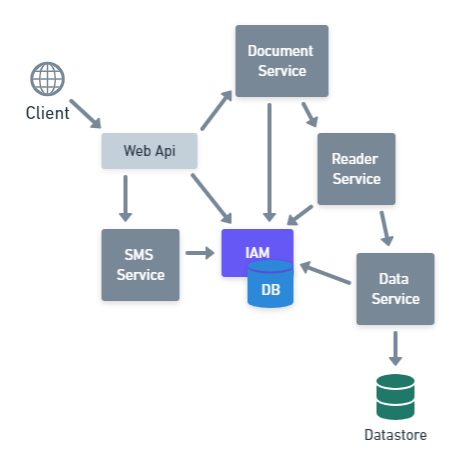
\includegraphics[width=\columnwidth]{images/service_depth.png}
    \caption{Deep MSA problem}
    \label{fig:deepMSA}
\end{figure}

The problem with ``service depth'' is not the performance
impact of computation itself in a work unit, but the general impact
on the overall system when chaining subsequent units together.
\autoref{fig:deepMSA} shows such a scenario. For the sake of
simplicity, let us assume that each call in \autoref{fig:deepMSA}
(i.e. Client to Api, Api to IAM\footnote{\label{fn:IAM}Identity and Access Management},
Service to Service, and Service to Datastore) takes \texttt{100ms}.

The assumed time contains computation, transformation from and to
the transport protocol and the round trip.
The basic idea is to show the performance impact when chaining services
into a ``deep system''.
With the given description, let us consider the following two scenarios:

\begin{enumerate}
    \item \textit{Client sends a SMS}:
    Client $\rightarrow$ Api $\rightarrow$ SMS Service. Api and SMS Service make
    a credentials check at the IAM\textsuperscript{\ref{fn:IAM}}.
    The successful response to the client
    is delivered after: $4 * 100ms = 400ms$
    \item \textit{Client requests a document}:
    Client $\rightarrow$ Api $\rightarrow$ Document Service $\rightarrow$
    Reader Service $\rightarrow$ Data Service $\rightarrow$ Data Store.
    All services check the credentials with the IAM\textsuperscript{\ref{fn:IAM}}.
    The successful response to the client
    is delivered after: $100ms \text{(Client)} + 4*100ms \text{(IAM)}
    + 3*100ms \text{(Services)} + 100ms \text{(DB)} = 900ms$
\end{enumerate}

A possible solution to this particular problem is to plan
the microservices and the corresponding architecture accordingly.
Frequent review of the current architecture and refactoring \cite{zio:ARforCloud}
if needed are key to prevent too deep services. This can happen
in a very agile way since one of the basic goals of MSA is
to have fast deployable artifacts.

The usage of synchronous HTTP calls will definitely result
in a performance penalty. Systems like ``Google PubSub'' could help
mitigate this bottleneck and create the possibility to scale
instances of microservices on the horizontal scale.
Furthermore, Kubernetes, among other orchestration platforms, provide developers with
battle-proof tools to scale services with load-balancing features
such as ``services'' which map to instances of the given services.

The statement about hardware is accurate. Depending on the hardware,
the performance of the whole MSA based system will vary. For example,
let us consider a microservice that was developed with
PHP\footnote{\url{https://www.php.net/}}. Depending on the used framework,
PHP loads the \texttt{*.php} script files for each and every call that
is made to the application. Since those script files are not cached
in memory or any compiled form, when the underlying hardware contains
storage with normal hard disk drives instead of solid state disks,
the performance impact is huge. On the other hand, a compiled application
like a C\# Web-Application does load itself into the memory of the
container and does not have the need to load some files for each request.

The second challenge \textit{Providing security at runtime} does
describe some of the current problems. Security is a hard topic
on itself and in conjunction with MSA, it does not get any easier.
Several patterns exist, that can provide some mechanism of security,
but as always, there is no silver bullet. A good strategy to
authenticate and authorize calls made from a source would be the usage
of OpenID Connect (OIDC) \cite{Siriwardena:OIDC}. OIDC enables
a system to have a centralized user and access management. The
calls are authenticated with a token and each microservice can check
if the call is authenticated and valid or not. As for authorization,
the central identity server can provide endpoints to fetch roles
or other means of authorization logic to check if the call is allowed
in the given microservice with the provided token.

\subsubsection{Quality attributes}

The SMS does a good job at showing the positive and negative
statements of the relevant studies. The comparison and categorization
is well done and gives an overview which topics contain solutions
for non-MSA-problems and which problems are newly introduced by
MSA and DevOps itself. The most important statement here is the security
concern. Security is and will be a part of any public application
and therefore is a central topic.

\subsubsection{Tool support}

The validity of this part of the results is questionable.
The listed and found tools over all the regarded publications mix
use-cases of various tools. As an example, ``Jira'' is listed
as monitoring tool, but I would argue, that ``Jira'' is definitely
not a tool for monitoring, regardless of the topic or the context.
The results show the provide tools in the stated topics, but the
discussion could have critically analyzed the tools and their positions
in the categories. Another example is ``Filebeat'', which is listed under
``Security Services and Tools''. But Filebeat should be listed under
monitoring or logging tools since it reads files produced by a service
and sends them to an ELK\footnote{\url{https://www.elastic.co/elastic-stack}} stack.
Filebeat itself does nothing in terms of security, it is a log analyzer.

Furthermore, the vast majority of the listed tools are ``Enterprise Tools''.
This does not necessarily mean they are not worth a try,
but they tend to be aged and not created according to the
newest and latest patterns and practices.

There are many open-source industry driven tools missing. Many
modern companies use newer and more state-of-the-art tools.
A few examples:

\begin{itemize}
    \item \textbf{Clair} \textit{Security}:
    A security scanner for containerized software that can statically analyze
    built containers for issues
    (\url{https://blogs.vmware.com/opensource/2019/10/31/clair-container-security/})
    \item \textbf{Jaeger} \textit{Monitoring}:
    Open-Source tracing tool that enables the developers to trace calls
    trough a complex system from end to end
    (\url{https://www.jaegertracing.io/})
    \item \textbf{GitHub Actions} \textit{CI}: The automated continuous integration
    platform from github
    \item \textbf{Gitlab CI} \textit{CI}: The automated continuous intregration
    platform from gitlab
    \item \textbf{ArgoCD} \textit{Configuration Management}: ArgoCD is an
    application that manages applications declaratively (GitOps pattern).
    Instead of using a CI pipeline to deploy an application to a cluster,
    the CI pipeline only creates the artifact (e.g. a Docker image) and publishes
    it somewhere. Then the pipeline can update the declarative description
    of the application with the new version of the image and Argo will
    be aware of the change and therefore will deploy the new image
    (\url{https://argoproj.github.io/argo-cd/})
\end{itemize}

The industry has produced many more tools that solve some of the stated
problems during the past years. Most of them were only mentioned or described
in gray literature.
